\documentclass[a4paper]{article}

%% Language and font encodings
\usepackage[english]{babel}
\usepackage[utf8x]{inputenc}
\usepackage[T1]{fontenc}

%% Sets page size and margins
\usepackage[a4paper,top=3cm,bottom=2cm,left=2cm,right=2cm,marginparwidth=2cm]{geometry}

%% Useful packages
\usepackage{amsmath}
\usepackage{amsfonts}
\usepackage{bbm}
\usepackage{graphicx}
\usepackage[colorinlistoftodos]{todonotes}
\usepackage[colorlinks=true, allcolors=blue]{hyperref}
\usepackage{float}
\usepackage{enumerate}
\usepackage[export]{adjustbox}
\usepackage{mathrsfs}
\usepackage{subcaption}

\usepackage{tikz}
\tikzset{
    vertex/.style={circle,draw,minimum size=1.5em},
    edge/.style={->,> = latex'}
}

\title{Stochastic Processes}
\author{Kevin Chang}

\graphicspath{ {./images/} }

\begin{document}
\maketitle

\section{Laplace Transform}
\begin{itemize}
    \item $\mathcal{L}\{f\}(s) = \int_0^\infty f(t) e^{-st} dt$
    \item Property
        \begin{itemize}
            \item $tf(t) \leftrightarrow -F'(s)$
            \item $\frac{f(t)}{t} \leftrightarrow \int_s^\infty F(\sigma) d \sigma$
            \item $f'(t) \leftrightarrow sF(s) - f(0^-)$
            \item $\int_0^t f(\tau) d\tau \leftrightarrow \frac{F(s)}{s}$
            \item $e^{at}f(t) \leftrightarrow F(s-a)$
            \item $f(t-a)u(t-a) \leftrightarrow e^{-at}F(s)$
        \end{itemize}
\end{itemize}

\section{Moment Generating Function}
\begin{itemize}
    \item Moment Generating Function: $\mathbb{E}[e^{tX}]$
        \begin{itemize}
            \item Property:
                \begin{itemize}
                    \item $\mathbb{E}[e^{tX}] = \int_{-\infty}^\infty e^{tx} f_X(x) dx$
                    \item $\mathbb{E}[e^{tX}] = \sum_{k=0}^\infty \mathit{E}[X^k] \frac{t^k}{k!}$
                        \begin{itemize}
                            \item $e^{tx} = \sum_{k=0}^\infty \frac{(tx)^k}{k!}$
                            \item $\mathit{E}[e^{tX}] = \mathit{E}[\sum_{k=0}^\infty \frac{(tX)^k}{k!}] = \sum_{k=0}^\infty \mathit{E}[X^k] \frac{t^k}{k!}$
                        \end{itemize}
                    \item $\frac{d\mathbb{E}[e^{tX}]}{dt} = \mathbb{E}[X]$
                    \item $\mathbb{E}[e^{t(aX+b)}] = e^tb\mathbb{E}[e^{taX}]$
                    \item Not all random variables have Moment generating function
                \end{itemize}
        \end{itemize}
    \item Characteristic Function: $\mathbb{E}[e^{itX}]$
        \begin{itemize}
            \item Property:
                \begin{itemize}
                    \item All random variables have Moment generating function
                \end{itemize}
        \end{itemize}
    \item Joint Moment Generating Function: $G(x, y) = \mathbb{E}[e^{xX}e^{yY}]$
    \item Property:
        \begin{itemize}
            \item (Joint) moment generating funciton uniquely determines the (joint) CDF
        \end{itemize}
    \item Example
        \begin{itemize}
            \item Trapped miner's random walk
                \begin{itemize}
                    \item Miner has probability of $\frac{1}{3}$ to waste 3 hours in vain, $\frac{1}{3}$ to waste 5 hours in vain, and $\frac{1}{3}$ to spend 2 hours to go out of the mine.
                    \item $X$ is the random variables of the hours to go out of the mine
                    \item $Y_i$ is the random variables of the hours for the $i$-th action.
                    \item $\mathbb{E}[e^{tX}] = \mathbb{E}[e^{tX}|Y_1 = 2] + \mathbb{E}[e^{tX}|Y_1 = 3] + \mathbb{E}[e^{tX}|Y_1 = 5]$

                        $= \mathbb{E}[e^{2t}] + \mathbb{E}[e^{t(X+3)}] + \mathbb{E}[e^{t(X+5)}]$
                    \item Find expectation and variance by joint moment generating function
                \end{itemize}
        \end{itemize}
\end{itemize}

\section{Expectation}
\begin{itemize}
    \item $N$ i.i.d. events, when $N$ is a random variable
        \begin{itemize}
            \item Suppose $N$ is a integer random variable
            \item Suppose $X_1, \dots, X_i, \dots, X_N$ are i.i.d random variables with mean $\mu$ and variance $\sigma^2$
            \item $Y = \sum_{i = 1}^N X_i$
            \item $\mathbb{E}[Y] = \mathbb{E}[N] \mu$
                \begin{itemize}
                    \item $\mathbb{E}[Y] = \sum_{n = 1}^\infty \mathbb{E}[\sum_{i = 1}^N X_i|N=n] P[N=n]$

                        $= \mu \times \sum_{n=1}^\infty n P[N=n] = \mathbb{E}[N] \mu$
                \end{itemize}
            \item $\mathbb{E}[Y^2] = \mathbb{E}[N] \mathbb{E}[X^2] + \mathbb{E}[N^2] \mu^2 - \mathbb{E}[N] \mu^2$
                \begin{itemize}
                    \item $\mathbb{E}[Y^2] = \sum_{n = 1}^\infty \mathbb{E}[(\sum_{i = 1}^N X_i)^2|N=n] P[N=n]$
                        $= \sum_{n = 1}^\infty (n \mathbb{E}[X_i^2] + n(n-1)\mu^2) P[N=n]$

                        $= \mathbb{E}[N] \mathbb{E}[X^2] + \mathbb{E}[N^2] \mu^2 - \mathbb{E}[N] \mu^2$
                \end{itemize}
            \item $\mathit{Var}(Y) = \mathbb{E}[N]\sigma^2 + \mathit{Var}(N)\mu^2$
        \end{itemize}
    \item Expectation by $P[X>x]$
        \begin{itemize}
            \item $\mathbb{E}[X] = \sum_x P[X > x]$, when $X$ is a non-negative discrete random variable
                \begin{itemize}
                    \item $\mathbb{E}[X] = \sum_{x=0}^\infty x P[X = x] = \sum_{x=0}^\infty \sum_{y=0}^{x-1} P[X = x] = \sum_{y=0}^\infty \sum_{x=y + 1}^\infty P[X = x] = \sum_{y = 0}^\infty P[X > y]$
                \end{itemize}
            \item $\mathbb{E}[X] = \int_0^\infty P[X > x] dx$, when $X$ is a non-negative continuous random variable
                \begin{itemize}
                    \item $\mathbb{E}[X] = \int_0^\infty x f_X(x) dx = \int_0^\infty \int_0^x f_X(x) dy dx = \int_0^\infty \int_y^\infty f_X(x) dx dy = \int_0^\infty P[X > y] dy$
                \end{itemize}
        \end{itemize}
\end{itemize}

\section{Inequality}
\begin{itemize}
    \item Markov Inequality

        Definition:
        \begin{itemize}
            \item Suppose $X \geq 0$, then $P[X \geq \epsilon] \leq \frac{\mathbb{E}[X]}{\epsilon}$
        \end{itemize}

        Proof:
        \begin{enumerate}
            \item $\mathbb{E}[X] = \int_0^\infty x f_X(x) \geq \int_\epsilon^\infty x f_X(x) \geq \epsilon \int_\epsilon^\infty f_X(x) = \epsilon P[X \geq \epsilon]$
            \item $X(\omega) \geq \epsilon \mathbbm{1}_{X(\omega) \geq \epsilon}, \forall \omega \in S$
                \begin{itemize}
                    \item Calculate expectation on both side.
                    \item $\mathbb{E}[X] \geq \epsilon P[X \geq \epsilon]$
                \end{itemize}
        \end{enumerate}
        Property:
        \begin{itemize}
            \item The equality happens when $P[X=k] = 0, \forall k \not \in \{0, \epsilon\}$.
        \end{itemize}
    \item Chebyshev Inequality

        Definition:
        \begin{itemize}
            \item Suppose $m = \mathbb{E}[X], \sigma^2 = \mathit{Var}(X)$, then $P[|X - m| \geq \epsilon] \leq \frac{\sigma^2}{\epsilon^2}$
        \end{itemize}
        Proof:
        \begin{itemize}
            \item $P[|X - m| \geq \epsilon] = P[(X - m)^2 \geq \epsilon^2]$
            \item $P[(X - m)^2 \geq \epsilon^2] \leq \frac{\mathbb{E}[(X-m)^2]}{\epsilon^2}$ (by Markov Inequality)
        \end{itemize}
        Property:
        \begin{itemize}
            \item The equality happens when $P[X = k] = 0, \forall k \not \in \{m - \epsilon , m , m + \epsilon\}$.
            \item Might be tighter than Markov Inequality since it requires $m, \sigma$
        \end{itemize}
    \item Chernoff Inequality

        Definition:
        \begin{itemize}
            \item Suppose $X_1, \dots, X_n$ are independent identically distributed Bernoulli random variable with probability $p$ and $X = \sum_{i=1}^n X_i$
            \item $P[X \geq \epsilon] \leq \frac{(pe^{t} + 1 - p)^n}{e^{t\epsilon}} \leq \frac{e^{np(e^{t} - 1)}}{e^{t\epsilon}}$
                \begin{itemize}
                    \item $P[X \geq \epsilon] = P[e^{tX} \geq e^{t\epsilon}] \leq \frac{E[e^{tX}]}{e^{t\epsilon}} = \frac{(E[e^{tX_i}])^n}{e^{t\epsilon}} = \frac{(pe^{t} + 1 - p)^n}{e^{t\epsilon}} \leq \frac{e^{np(e^{t} - 1)}}{e^{t\epsilon}}$
                \end{itemize}
            \item $P[X \geq np(1 + \epsilon)] \leq (\frac{e^{\epsilon}}{(1+\epsilon)^{1 + \epsilon}})^{np} \leq \left\{ \begin{array}{ll} e^{\frac{-\epsilon^2 np}{3}} & \text{ if } 0 \leq \epsilon \leq 1 \\ e^{\frac{-\epsilon^2 np}{(2 + \epsilon)}} & \text{ if } \epsilon \geq 1 \end{array} \right.$
                \begin{itemize}
                    \item Substitude $\epsilon$ with $np(1+\epsilon)$
                    \item Substitude $t$ with $\log(1+\epsilon)$
                    \item the last inequality is without proof
                \end{itemize}
            \item $P[X \leq \epsilon] \leq \frac{(pe^{t} + 1 - p)^n}{e^{t\epsilon}} \leq \frac{e^{np(e^{t} - 1)}}{e^{t\epsilon}}$
                \begin{itemize}
                    \item $P[X \leq \epsilon] = P[e^{-tX} \geq e^{-t\epsilon}] \leq \frac{E[e^{-tX}]}{e^{-t\epsilon}} = \frac{(E[e^{-tX_i}])^n}{e^{-t\epsilon}} = \frac{(pe^{-t} + 1 - p)^n}{e^{-t\epsilon}} \leq \frac{e^{np(e^{-t} - 1)}}{e^{-t\epsilon}}$
                \end{itemize}
            \item $P[X \leq np(1 - \epsilon)] \leq (\frac{e^{-\epsilon}}{(1-\epsilon)^{1 - \epsilon}})^{np} \leq e^{\frac{-\epsilon^2 np}{2}}$
                \begin{itemize}
                    \item Substitude $\epsilon$ with $np(1-\epsilon)$
                    \item Substitude $t$ with $- \log(1-\epsilon)$
                    \item the last inequality is without proof
                \end{itemize}
        \end{itemize}
    \item Chernoff/ Hoeffding Lemma

        Definition:
        \begin{itemize}
            \item Suppose $X_1, \dots, X_n$ are independent distributed random variable and $a_i \leq X_i \leq b_i$
            \item Suppose $X = \sum_{i=1}^n X_i$ and $\mu = \mathbb{E}[X]$
            \item $P[|X-\mu| \geq \epsilon] \leq 2 e^{\frac{-2\epsilon^2}{\sum_{i=1}^n(b_i - a_i)^2}}$ without proof
        \end{itemize}
    \item Application:
        \begin{itemize}
            \item Balls in Bins

                Definition: Throw $n$ balls into $n$ bins, find bounds for the maximum number of balls in all bins
                \begin{itemize}
                    \item $P[\text{ maximum number of balls in all bins } \geq \epsilon]$

                        $= P[\cup_{i=1}^n \text{ number of balls in $i$-th bin } \geq \epsilon]$

                        $\leq n \times P[\text{ number of balls in one bin } \geq \epsilon]$
                    \item By Markov inequality:
                        \begin{itemize}
                            \item $P[\text{ number of balls in one bin } \geq \epsilon] \leq \frac{1}{\epsilon} \rightarrow$ useless
                        \end{itemize}
                    \item By Chebyshev inequality:
                        \begin{itemize}
                            \item $P[\text{ number of balls in one bin } \geq \epsilon] \leq \frac{(1-\frac{1}{n})}{\epsilon^2}$
                            \item $P[\text{ maximum number of balls in all bins } \geq n^{\frac{1}{2} + \epsilon}] \leq \frac{(1-\frac{1}{n})}{n^{2\epsilon}}$
                            \item when $n \rightarrow \infty$, the maximum number of balls should less than $n^{\frac{1}{2} + \epsilon}$
                        \end{itemize}
                    \item By Chernoff inequality:
                        \begin{itemize}
                            \item $P[\text{ number of balls in one bin } \geq 2 \log n] \leq \frac{e^{np(e^{t} - 1)}}{n^{2t}}$
                            \item $P[\text{ maximum number of balls in all bins } \geq 2 \log n] \leq \frac{e^{np(e^{t} - 1)}}{n^{2t - 1}}$
                            \item when $t$ is a constant $\geq 0.5$ and $n \rightarrow \infty$, the maximum number of balls should less than $2 \log n$
                        \end{itemize}
                \end{itemize}
        \end{itemize}
\end{itemize}

\section{Law of Large Numbers}
\begin{itemize}
    \item $\{X_i\}_{i = 1}^\infty$ is a sequence of pairwise uncorrelated random variable with

        $\mathbb{E}[X_i] = m, \mathit{Var}(X_i) = \sigma_i^2$.
    \item $M_n = \frac{1}{n}\sum_{i = 1}^n X_i$
    \item $M_n \rightarrow m$ almost surely, in mean square and in probability.
\end{itemize}

\section{Memoryless}
\begin{itemize}
    \item Definition: $P[X > x_1 + x_2 | X > x_1] = P[X > x_2]$
    \item Property:
        \begin{itemize}
            \item Exponential random variable is the only continuous memoryless random variable
            \item Bernoulli random variable is the only discrete memoryless random variable
        \end{itemize}
\end{itemize}

\section{Famous Random Variable}
\begin{itemize}
    \item Poisson:

        $P[X=k] = \frac{\lambda^k}{k!}\exp(-\lambda)$

        $\mathbb{E}[X] = \sum_{k=0}^\infty k\frac{\lambda^k}{k!}\exp(-\lambda)$
        $= \sum_{k=0}^\infty \lambda \frac{\lambda^{k-1}}{(k-1)!}\exp(-\lambda) = \lambda$

        Interpretation:
        \begin{itemize}
            \item Cut total time into infinite period in Binomial random variable, $n \rightarrow \infty, p \rightarrow \frac{\lambda}{n}$

            \item $\rightarrow P[X=k] = \lim_{n\rightarrow \infty} \binom{n}{k}(\frac{\lambda}{n})^k(\frac{n-\lambda}{n})^{n-k} = \frac{\lambda^k}{k!}(1-\frac{\lambda}{n})^{n} = \frac{\lambda^k}{k!}\exp(-\lambda)$
        \end{itemize}
    \item Erlang:

        $f_X(x) = \frac{\lambda^n x^{n-1} e^{-\lambda x}}{(n-1)!}, \forall x \in \mathbb{R}$

        $\mathbb{E}[X] = \frac{n}{\lambda}$

        Interpretation:
        \begin{itemize}
            \item Suppose $X_1, X_2, ..., X_n$ are i.i.d exponential random variable with $\lambda$.
            \item $X = \sum_{i = 1}^n X_i$
            \item Proof by induction:

                Suppose $n = 2$, 
                $f_X(x) = \int_0^x \lambda e^{-\lambda t} \lambda e^{-\lambda(x - t)} dt$
                $= \lambda^2 x e^{-\lambda x}$
        \end{itemize}
\end{itemize}

\section{Stochastic Processes}
\begin{itemize}
    \item Stochastic Process: a collection of random variable

        Arrival Process: a sequence of arriving event in continuous time
\begin{figure} [H]
    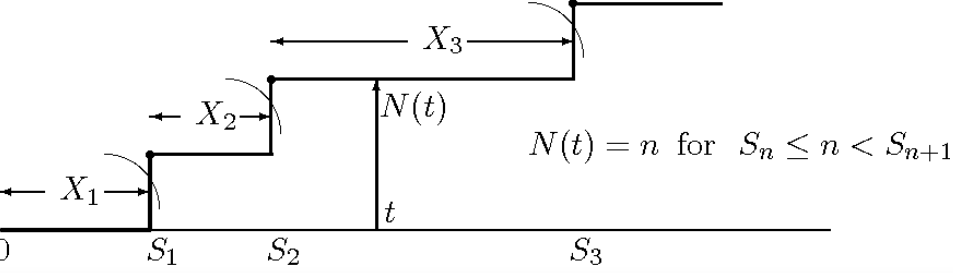
\includegraphics[width=0.5\linewidth, center]{image/arrival_process.png}
\end{figure}
        \begin{itemize}
            \item $X_i$: the time between the $i$-th event and the $i-1$-th event
            \item $S_i$: the time from start to $i$-th event
            \item $N(t)$: the number of the arrived event at time $t$
            \item $X$ and $S$ Relation:
                \begin{itemize}
                    \item $X_1 = S_1, X_i = S_i - S_{i-1}$
                \end{itemize}
            \item $N$ and $S$ Relation:
                \begin{itemize}
                    \item $N(t) < n \leftrightarrow S_{n+1} > t$
                    \item $N(t) \geq n \leftrightarrow S_n \leq t$
                    \item $N(t) = n \leftrightarrow S_n \leq t < S_{n+1}$
                    \item $N(t) = \max \{n: S_n \leq t\}$
                \end{itemize}
            \item Renewal Process: an arrival process with i.i.d $X_i$

                Delayed Renewal Process: the process becomes a renewal process after several arrivals

                $X_i$ Property
                \begin{itemize}
                    \item if $X_i$ is dependent on the interval states, then $X_i$ might be dependent on $X_{i-1} \rightarrow$ not renewal process
                \end{itemize}
                $S_i$ Property
                \begin{itemize}
                    \item $P[\lim_{n \rightarrow \infty} S_n = \infty] = 1$

                        Proof: $\lim_{n \rightarrow \infty} P[S_n = \infty] = \lim_{n \rightarrow \infty} P[\sum_{i = 1}^n X_n = n \times \mathbb{E}[X_i]] = 1$

                        Interpretation: infinite events do not take finite time
                \end{itemize}
                $N(t)$ Property
                \begin{itemize}
                    \item for any $t, P[N(t) < \infty] = 1$

                        Proof: $P[\lim_{n \rightarrow \infty} S_n = \infty] = 1 \rightarrow$ for any $t, P[\lim_{n \rightarrow \infty} S_{n+1} > t] = 1$

                        Interpretation: infinite events do not take finite time
                    \item $P[\lim_{t \rightarrow \infty} N(t) \rightarrow \infty] = 1$

                        Proof: if $P[\lim_{t \rightarrow \infty} N(t) = k] > 0 \rightarrow P[X_{k+1} = \infty] > 0$

                        Interpretation: finite events do not take infinite time
                    \item $P[\lim_{t \rightarrow \infty} \frac{N(t)}{t} = \frac{1}{\mathbb{E}[X_i]}] = 1$

                        Proof: $P[\lim_{t \rightarrow \infty} \frac{N(t)}{S_{N(t) + 1}} \leq \lim_{t \rightarrow \infty} \frac{N(t)}{t}] = 1$ and $P[\lim_{t \rightarrow \infty} \frac{N(t)}{S_{N(t) + 1}} = \frac{1}{\mathbb{E}[X_i]}] = 1$

                        $P[\lim_{t \rightarrow \infty} \frac{N(t)}{t} \leq \lim_{t \rightarrow \infty} \frac{N(t)}{S_{N(t)}}] = 1$ and $P[\lim_{t \rightarrow \infty} \frac{N(t)}{S_{N(t)}} = \frac{1}{\mathbb{E}[X_i]}] = 1$
                \end{itemize}
                Inspection Paradox
                \begin{itemize}
                    \item $\mathbb{E}[X_{N(t) + 1}] \geq \mathbb{E}[X_i]$: inspection paradox

                        Interpretation:
                        \begin{itemize}
                            \item $f_{X_{N(t)+1}}(x) = \lambda x f_{X_i}(x)$
                            \item when selecting $t$ with equal probability, we tend to choose $X_i$ with longer period
                        \end{itemize}
                    \item $P[\lim_{t \rightarrow \infty} \frac{1}{t} \int_0^t (S_{N(t) + 1} - s) ds = \frac{\mathbb{E}[X_i^2]}{2\mathbb{E}[X_i]}] = 1$

                        Proof:

                        $P[\lim_{t \rightarrow \infty} \frac{1}{t} \sum_{i = i}^{N(t)} \frac{\mathbb{E}[X_i^2]}{2} \leq \lim_{t \rightarrow \infty} \frac{1}{t} \int_0^t (S_{N(t) + 1} - s) ds] = 1$ and $P[\lim_{t \rightarrow \infty} \frac{1}{t} \sum_{i = i}^{N(t)} \frac{\mathbb{E}[X_i^2]}{2} = \frac{\mathbb{E}[X_i^2]}{2\mathbb{E}[X_i]}] = 1$

                        $P[\lim_{t \rightarrow \infty} \frac{1}{t} \int_0^t (S_{N(t) + 1} - s) ds \leq \lim_{t \rightarrow \infty} \frac{1}{t} \sum_{i = i}^{N(t) + 1} \frac{\mathbb{E}[X_i^2]}{2}] = 1$ and $P[\lim_{t \rightarrow \infty} \frac{1}{t} \sum_{i = i}^{N(t) + 1} \frac{\mathbb{E}[X_i^2]}{2} = \frac{\mathbb{E}[X_i^2]}{2\mathbb{E}[X_i]}] = 1$
                    \item $P[\lim_{t \rightarrow \infty} \frac{1}{t} \int_0^t (s - S_{N(t)}) ds = \frac{\mathbb{E}[X_i^2]}{2\mathbb{E}[X_i]}] = 1$

                        Proof: similar to above
                    \item $P[\lim_{t \rightarrow \infty} \frac{1}{t} \int_0^t X_{N(t)} ds = \frac{\mathbb{E}[X_i^2]}{\mathbb{E}[X_i]}] = 1$

                        Proof: $P[\lim_{t \rightarrow \infty} \frac{1}{t} \int_0^t X_{N(t)} ds = \lim_{t \rightarrow \infty} \frac{1}{t} \int_0^t (S_{N(t) + 1} - S_{N(t)}) ds] = 1$
                    \item $\mathbb{E}[X_{N(t) + 1}] = \frac{\mathbb{E}[X_i^2]}{\mathbb{E}[X_i]}$

                        Proof: $P[\lim_{t \rightarrow \infty} \frac{1}{t} \int_0^t X_{N(t)} ds = \frac{\mathbb{E}[X_i^2]}{\mathbb{E}[X_i]}] = P[\mathbb{E}[X_{N(t) + 1}] = \frac{\mathbb{E}[X_i^2]}{\mathbb{E}[X_i]}] = 1$
                \end{itemize}
                Central Limit Theorem
                \begin{itemize}
                    \item $\mu = \mathbb{E}[X_i]$
                    \item $\sigma = \sqrt{\mathit{Var}(X_i)}$
                    \item $Z \sim$ Normal(0,1)
                    \item $\lim_{t \rightarrow \infty} P[N(t) \leq \frac{t}{\mu} + k \frac{\sigma \sqrt{t}}{\sqrt{\mu}^3}] = P[Z \leq k]$

                        Proof:
                        \begin{enumerate}
                            \item Suppose $n(t) = \frac{t}{\mu} + k \frac{\sigma \sqrt{t}}{\sqrt{\mu}^3}$
                            \item $P[N(t) \geq n(t)] = P[S_{n(t)} \leq t] = P[\frac{S_{n(t)} - n\mu}{\sigma \sqrt{n}} \leq \frac{t - n\mu}{\sigma \sqrt{n}}]$.
                            \item When $t \rightarrow \infty$, $\frac{t - n\mu}{\sigma \sqrt{n}} \rightarrow k$
                            \item By law of large number, $\lim_{t \rightarrow \infty} P[\frac{S_{n(t)} - n\mu}{\sigma \sqrt{n}} \leq k] = P[Z \leq k]$
                        \end{enumerate}
                        Interpretation:
                        \begin{itemize}
                            \item $\frac{t}{\mu}$ is approximately the mean of $N(t)$
                            \item $k \frac{\sigma \sqrt{t}}{\sqrt{\mu}^3}$ is $k\sigma \sqrt{n}$ after dividing by $\mu$, the ratio between $t$ and $N(t)$ and changing $n$ with $\frac{t}{\mu}$
                        \end{itemize}
                \end{itemize}
                Wald's Identity
                \begin{itemize}
                    \item Stopping Times: a random variable $\tau$ s.t. $\{\tau = n\}$ is independent of $\{X_i\}_{i=n+1}^\infty$
                    \item Stopping Condition: a condition to stop if we can consider $\tau = \min\{n: \text{ condition}(n) = \top \}$
                    \item Example: $N(t) + 1$ is a stopping times and can be consider $N(t) + 1 = \min\{n: S_n > t\}$
                    \item $\mathbb{E}[\sum_{i=1}^\tau X_i] = \mathbb{E}[\tau] \mathbb{E}[X_i]$ if $\mathbb{E}[X_i] < \infty$ and $\mathbb{E}[N] < \infty$

                        Proof:
                        \begin{enumerate}
                            \item $\mathbb{E}[\sum_{i=1}^\tau X_i] = \sum_{i=1}^\infty \mathbb{E}[X_i \times \mathbbm{1}_{i\leq \tau}]$ (by Fubin's Theorem without proof)

                               (if $\mathbb{E}[X_i] < \infty$ and $\mathbb{E}[N] < \infty$)
                            \item $\sum_{i=1}^\infty \mathbb{E}[X_i \times \mathbbm{1}_{i\leq \tau}] = \mathbb{E}[X_i] \sum_{i=1}^\infty \mathbb{E}[\mathbbm{1}_{i\leq \tau}]$ (by $P[\tau \geq i] = 1 - P[\tau < i]$ is independent of $X_i$)
                            \item $\mathbb{E}[X_i] \sum_{i=1}^\infty \mathbb{E}[\mathbbm{1}_{i\leq \tau}] = \mathbb{E}[\tau] \mathbb{E}[X_i]$
                        \end{enumerate}
                    \item $\lim_{t \rightarrow \infty} \frac{\mathbb{E}[N(t)]}{t} = \frac{1}{\mathbb{E}[X_i]}$

                        Proof:
                        \begin{itemize}
                            \item Suppose $\mu = \mathbb{E}[X_i]$
                            \item $\frac{\mathbb{E}[N(t)]}{t} = \frac{\mathbb{E}[S_{N(t) + 1}]}{t \times \mu} - \frac{1}{t}$ (by considering $N(t) + 1$ as the stopping time)
                            \item $\lim_{t \rightarrow \infty} \frac{\mathbb{E}[N(t)]}{t} \geq \frac{1}{\mu}$ (by $\mathbb{E}[S_{N(t) + 1}] > t$)
                            \item Suppose $\hat{X}_n = \min\{X_n, T\}$, where $T$ is a constant
                            \item $\frac{\mathbb{E}[N(t)]}{t} \leq \frac{\mathbb{E}[\hat{N}(t)]}{t} = \frac{\mathbb{E}[S_{\hat{N}(t) + 1}]}{t \times \hat{\mu}} - \frac{1}{t} \leq \frac{t+T}{t \times \hat{\mu}} - \frac{1}{t}$
                            \item $\lim_{n = \sqrt{t}, t \rightarrow \infty} \frac{\mathbb{E}[N(t)]}{t} \leq \frac{1}{\mu}$
                        \end{itemize}
                \end{itemize}
                Blackwell's Theorem
                \begin{itemize}
                    \item $\mathbb{E}[N(t)] = F_{X_i}(t) + \int_0^t \mathbb{E}[N(t-x)] f_{X_i}(t) dt$

                        Proof:
                        $\mathbb{E}[N(t)] = \int_0^t \mathbb{E}[N(t)|X_1 = x] f_{X_1}(x) dx$

                        $= \int_0^t \mathbb{E}[N(t-x) + 1] f_{X_1}(x) dx$
                        $= F_{X_i}(t) + \int_0^t \mathbb{E}[N(t-x)] f_{X_i}(t) dt$
                    \item $\mathcal{L}\{\mathbb{E}[N(t)]\}(s) = \frac{\mathcal{L}\{f_{X_i}\}(s)}{s(1 - \mathcal{L}\{f_{X_i}\}(s))}$

                        Proof: Laplace transform both sides
                    \item Lattice/ Non-Lattice: $N(t)$ is lattice iff $X_i$ only takes on values that are $nd, n \in \mathbb{N}, d \in \mathbb{R}$
                    \item For a non-lattice process: $\lim_{t \rightarrow \infty} \mathbb{E}[N(t + \delta) - N(t)] = \frac{\delta}{\mathbb{E}[X_i]}$, for any $\delta$

                        Proof: Without Proof

                        Interpretation: $\mathbb{E}[N(t)]$ will converge to be linear
                    \item For a lattice process and period $d$: $\lim_{n \rightarrow \infty} \mathbb{E}[\text{\# events at $t = nd$}] = \frac{d}{\mathbb{E}[X_i]}$

                        Proof: Without Proof

                        Interpretation: $\mathbb{E}[N(t)]$ will converge to be stairs with width $d$ and height $\frac{d}{\mathbb{E}[X_i]}$
                \end{itemize}
            \item Renewal-Reward Process:

                Definition
                \begin{itemize}
                    \item A renewal process $N(t)$ and $\{R_i\}_{i = 1}^\infty$ such that $(X_i, R_i)$ are i.i.d.

                        ($X_i, R_j, i \not = j$ are independent, but $X_i, R_i$ might be dependent)
                \end{itemize}
                Property
                \begin{itemize}
                    \item $P[\lim_{t \rightarrow \infty} \frac{1}{t} \sum_{i=1}^{N(t)} R_i = \frac{\mathbb{E}[R_i]}{\mathbb{E}[X_i]}] = 1$

                        Proof: $P[\lim_{t \rightarrow \infty} \frac{1}{t} \sum_{i=1}^{N(t)} R_i = \lim_{t \rightarrow \infty} \sum_{i=1}^{N(t)} \frac{R_i}{N(t)} \times \lim_{t \rightarrow \infty} \frac{N(t)}{t}] = 1$
                \end{itemize}
            \item Poisson Process: a renewal process with $X_i \sim \text{Exponential}(\lambda)$

                $S_i$ Property
                \begin{itemize}
                    \item $S_i$ is an Erlang random variable

                        Erlang is the sum of the Exponential random variables
                    \item Joint Distribution $f_{S_1, \dots, S_n}(s_1, \dots, s_n) = \lambda^n e^{-\lambda s_n}$

                        Prove by induction.

                        Induce by $f_{S_1, \dots, S_n}(s_1, \dots, s_n) = f_{S_1, \dots, S_{n-1}}(s_1, \dots, s_{n-1}) \times f_{S_n | S_1, \dots, S_{n-1}}(s_n, s_1, \dots, s_{n-1})$
                \end{itemize}
                $N(t)$ Property
                \begin{itemize}
                    \item $N(t) \sim \text{Poisson}(\lambda t), P[N(t) = n] = \frac{(\lambda t)^n}{n!}e^{-\lambda t}$ 

                        Prove by $P[N(t) = n] = P[S_n \leq t \text{ and } S_{n+1} > t]$
                    \item Conditioned on $N(t) = n$, the set of arrival times $\{s_1, \dots, s_n\}$ have the same distribution with a set of $n$ sorted i.i.d. Uniform$(0, t)$ random variables

                        Prove by $f_{S_1, \dots, S_n | N(t)}(s_1, \dots, s_n, n) = \frac{f_{S_1, \dots, S_n}(s_1, \dots, s_n) P[X_{n+1} > t - s_n]}{P[N(t) = n]} = \frac{n!}{t^n}$
                \end{itemize}
                Property
                \begin{itemize}
                    \item $Z$ is the interval from $t$ to the first arrival $\rightarrow Z$ is exponential random variable with same $\lambda$ and independent of $N(t)$ and the arrival time before $t$

                        Proof:

                        $P[Z > z] = \sum_{n = 0}^\infty \int_0^\infty \dots \int_0^\infty P[Z>z|N(t) = n, S_1 = s_1, \dots, S_n = s_n] ds_1 \dots ds_n$

                        $= \sum_{n = 0}^\infty \int_0^\infty \dots \int_0^\infty P[X_{n+1}>z+t-s_n|N(t) = n, S_1 = s_1, \dots, S_n = s_n] ds_1 \dots ds_n$

                        $= \sum_{n = 0}^\infty \int_0^\infty \dots \int_0^\infty P[X_{n+1}>z+t-s_n|X_{n+1} > t-s_n] ds_1 \dots ds_n = e^{-\lambda z}$
                    \item Stationary Increments: $N(t_1 + t_2) - N(t_1)$ and $N(t_2)$ share the same distribution

                        Without Proof
                    \item Independent Increments: $\forall 0 < t_1 < t_2 < \dots, t_k, N(t_1), N(t_2) - N(t_1), \dots$ are independent

                        Without Proof
                    \item Any arrival process with stationary and independent increments must be a Poisson process

                        Without Proof
                \end{itemize}
                Exercise
                \begin{itemize}
                    \item $\mathbb{E}[S_i|N(t) = n] = \frac{t \times i}{n+1}$
                        \begin{itemize}
                            \item $\mathbb{E}[S_i|N(t) = n] = i \times \mathbb{E}[X_1|N(t) = n] = i \int_0^t \int_0^{s_n} \dots \int_0^{s_2} s_1 \times \frac{n!}{t^n} ds_1 \dots ds_{n-1} ds_n = \frac{t \times i}{n+1}$
                        \end{itemize}
                    \item $\mathbb{E}[\sum_{i=0}^{N(t)} S_i] = \frac{\lambda t^2}{2}$
                        \begin{itemize}
                            \item $\mathbb{E}[\sum_{i=0}^{N(t)} S_i] = \sum_{n = 0}^\infty \mathbb{E}[\sum_{i=0}^n S_i|N(t) = n]P[N(t) = n]$

                                $= \sum_{n = 0}^\infty \frac{nt}{2}P[N(t) = n] = \frac{\lambda t^2}{2}$
                        \end{itemize}
                \end{itemize}
                2D Poisson Process
                \begin{itemize}
                    \item Definition:
                        \begin{itemize}
                            \item For any region $R$: number of points in $R$ is a Poisson random variable
                            \item number of points in the non-overlapping region is independent
                        \end{itemize}
                \end{itemize}
                Combining Poisson Process
                \begin{itemize}
                    \item $N^1(t), N^2(t)$ are two independent Poisson process with $\lambda_1, \lambda_2$
                    \item $X_i$ is the first arrival of $X_i^1, X_i^2$
                    \item Property
                        \begin{itemize}
                            \item $X_i$ is independent of $\{X_i^1 < X_i^2\}$ and $\{X_i^1 > X_i^2\}$ 

                                Proof: $P[X_1^1 < X_1^2] = \frac{\lambda_1}{\lambda_1 + \lambda_2}$

                                $P[X_1 > x] = P[X_1^1 > x, X_1^2 > x] = e^{-(\lambda_1 + \lambda_2)x}$

                                $P[X_1 > x, X_1^1 < X_1^2] = P[X_1 > x]P[X_1^1 < X_1^2]$
                            \item $X_i$ is a Poisson Process with $\lambda = \lambda_1 + \lambda_2$
                            \item $\min(X_1, X_2)$ is an exponential random variable with $\lambda = \lambda_1 + \lambda_2$
                        \end{itemize}
                \end{itemize}
                Splitting Poisson Process
                \begin{itemize}
                    \item $N^1(t), N^2(t)$ are two independent Poisson process with $\lambda_1, \lambda_2$
                    \item $N(t)$ is a random process with $\lambda = \lambda_1 + \lambda_2$
                        \begin{itemize}
                            \item $N^{1*}(t)$ is the process of the first event

                                when $N(t)$ arrives consider it as first event with probability $\frac{\lambda_1}{\lambda_1 + \lambda_2}$
                            \item $N^{2*}(t)$ is the process of the second event

                                when $N(t)$ arrives consider it as second event with probability $\frac{\lambda_2}{\lambda_1 + \lambda_2}$
                        \end{itemize}
                    \item $N^i(t)$ and $N^{i*}(t)$ share the same distribution
                    \item Proof:
                        \begin{itemize}
                            \item $B_n(k)$ is a Binomial random variable with $p = \frac{\lambda_1}{\lambda_1 + \lambda_2}$
                            \item $P[N^{1*}(t) = m, N^{2*}(t) = n] = P[N(t) = m + n, B_{m+n}(m)] = P[N^1(t) = m, N^2(t) = n]$
                        \end{itemize}
                \end{itemize}
                Compound Poisson Process
                \begin{itemize}
                    \item $N(t)$ is a Poisson Process
                    \item $A_n$ is a sequence of cost
                    \item $A(t) = \sum_{n=0}^{N(t)} A_n$ is the summation of cost over Poisson Process
                \end{itemize}
                Non-Homogeneous Poisson Process
                \begin{itemize}
                    \item $N(t) - N(s) \sim$ Poisson$(\int_s^t \lambda(x) dx$
                \end{itemize}
                Queuing Theory
                \begin{itemize}
                    \item Definition: $\mathit{Arrival\_Process}/ \mathit{Service\_Process}/ \mathit{number\_of\_services}$
                        \begin{itemize}
                            \item $M$: memoryless (Poisson) process
                            \item $D$: deterministic process
                            \item $G$: general renewal process
                        \end{itemize}
                    \item $T$: the random variable of the processing time for each customer
                    \item $Y(t)$: number of cutomers in the service
                        \begin{itemize}
                            \item $Y(t) \sim$ Poisson$(\lambda \int_0^t P[T>x] dx)$
                            \item Proof:

                                Consider $Y(t)$ is a splitting Poisson Process. Since the distribution for the arrival given $N(t)$ is universal, the probability the arrival is still in service: $\frac{1}{t} \int_0^t P[T > t-x] dx = \frac{1}{t}\int_0^t P[T > x] dx$
                        \end{itemize}
                \end{itemize}
        \end{itemize}
\end{itemize}

\section{Markov Chain}
\begin{itemize}
    \item Definition
        \begin{itemize}
            \item Model with states and transition probability matrix
            \item States: $\{X_n\}_{n=0}^\infty$
            \item Transition Probability Matrix: $[P]_{ij} = P[X_{n+1} = j|X_n = i]$
        \end{itemize}
    \item Terminology
        \begin{itemize}
            \item $p^n = [P[X_n = 0], P[X_n = 1], \dots]^T$: distribution at step $n$
            \item $T_i = \min\{n \geq 1: X_n = i\}$: a random variable of the minimum time step to go to state $i$
            \item $f_{ij} = P[T_j < \infty | X_0 = i]$: the probability of starting at $i$ and ever reaching $j$
            \item $\mu_{ij} = \mathbb{E}[T_j | X_0 = i]$
            \item $i \rightarrow j$ iff $f_{ij} > 0$: $j$ is reachable from $i$ with probability greater than 0
            \item $N_i(n)$: number of visits to $i$ by time $n$
            \item Irreducible: $i \leftrightarrow j, \forall$ states $i, j$
            \item aperiodic: period of $X_n = i$ is 1, $\forall$ states $i$
        \end{itemize}
    \item Property
        \begin{itemize}
            \item Consider a given distribution as an event $\tau: [P[X_n = 0| \tau], P[X_n = 1| \tau], \dots]^T$
            \item Updating distribution
                \begin{itemize}
                    \item $p^n = p^0 P^n$
                \end{itemize}
            \item Markovian: transition probability depend only on current state
                \begin{itemize}
                    \item $P[X_{n+1} = j|X_n = i, \dots, X_0 = x_0] = [P]_{ij}$
                \end{itemize}
            \item Stationary Distribution: $p$ s.t. if $p^n = p \rightarrow p^{n+1} = p$

                Property from renewal process
                \begin{itemize}
                    \item consider $X_n = j$ as a event $\rightarrow$ Markov Chain becomes a delayed renewal process
                    \item If $i \leftrightarrow j$ and the model starts from $i$, then following holds
                    \item $P[\lim_{n \rightarrow \infty} \frac{N_j(n)}{n} = \frac{1}{\mu_{jj}}] = 1$
                    \item $\lim_{n \rightarrow \infty} \frac{\mathbb{E}[N_j(n)]}{n} = \frac{1}{\mu_{jj}}$
                    \item if the period of $X_n = j$ is $d \rightarrow \lim_{n \rightarrow \infty} p_j^{nd} = \frac{d}{\mu_{jj}}$
                \end{itemize}
                Theorem of an irreducible, aperiodic Markov Chain
                \begin{itemize}
                    \item Either
                        \begin{itemize}
                            \item All states have $\mu_{ii} = \infty$
                            \item All states have $\mu_{ii} < \infty$ and $p_i = \frac{1}{\mu_{ii}}$ is the unique stationary distribution
                        \end{itemize}
                    \item Proof
                        \begin{itemize}
                            \item From if the period of $X_n = j$ is $d \rightarrow \lim_{n \rightarrow \infty} p_j^{nd} = \frac{d}{\mu_{jj}}$

                            Proof: $\lim_{n \rightarrow \infty} p_j^{nd} = \lim_{n \rightarrow \infty} \mathbb{E}[\text{\# events at $nd$}]$
                        \end{itemize}
                \end{itemize}
                Theorem of an irreducible, aperiodic Markov Chain
                \begin{itemize}
                    \item All states have $\mu_{ii} < \infty$ and $p_i = \frac{1}{\mu_{ii}}$ is the unique stationary distribution
                \end{itemize}
                $p$ can be calculated as the eigenvector corresponds to eigenvalue $1$ of $P^T$
            \item Detailed Balance

                Definition:
                \begin{itemize}
                    \item Given a distribution $\pi$
                    \item $\pi_i P_{ij} = \pi_j P_{ji}, \forall i, j$
                \end{itemize}
                Property: 
                \begin{itemize}
                    \item distribution $\pi$ satisfying Detailed Balance is the stationary distribution $p$
                    \item symmetric transition probability matrix $\rightarrow$ uniform stationary distribution
                \end{itemize}
            \item Reversible

                Definition: A Markov Chain with stationary distribution $p$ is reversible if it satisfies detailed balance

                Interpretation
                \begin{itemize}
                    \item Transitions forward and backward in the stationary distribution have the same probability
                    \item $P[X_{n+1} = j| X_n = i] = P_{ij}$
                    \item $P[X_{n-1} = j| X_n = i] = \frac{P[X_{n-1} = j, X_n = i]}{P[X_n = i]} = \frac{p_j P_{ji}}{p_i} = P_{ij}$
                \end{itemize}
            \item Metropolis Update Rule

                Definition
                \begin{itemize}
                    \item Given a Markov Chain and distribution $p'$, find $P'$ such that $p'$ is the stationary distribution
                \end{itemize}
                Procedure
                \begin{itemize}
                    \item For each pair $(i,j)$, $P'_{ij} = P_{ij} \times \min\{1, \frac{p'_j P_{ji}}{p'_i P_{ij}} \}$
                    \item construct self loop to satisfy $\sum_j P'_{ij} = 1$
                \end{itemize}
                Proof
                \begin{itemize}
                    \item To satisfy detailed balance, for each pair $(i, j)$, we should set $p'_i P'_{ij} = \min\{p'_i P_{ij}, p'_j P_{ji}\}$ 
                \end{itemize}
            \item Distance between Probability Measure
                
                Definition:
                \begin{itemize}
                    \item Total Variation Distance between $P_1$ and $P_2$ is: $d_{\mathit{TV}}(P_1, P_2) = \frac{1}{2} \sum_{\omega} |P_1[\omega] - P_2[\omega]|$
                \end{itemize}
                Interpretation:
                \begin{itemize}
                    \item consider the distributions as events $\tau_1, \tau_2$
                    \item $P_i[\omega] = P[\omega|\tau_i]$
                    \item $d_{\mathit{TV}}(P_1, P_2) = \frac{1}{2} \sum_{\omega} |P[\omega | \tau_1] - P[\omega | \tau_2]|$
                        $= \sum_{\omega} |P[\omega \wedge \tau_1] - P[\omega \wedge \tau_2]|$
                \end{itemize}
            \item Mixing Time

                Definition
                \begin{itemize}
                    \item Mixing time $\tau$ is the least $t$ such that for all initial state $p^0$, $d_\mathit{TV}(p, p^0P^t) \leq \frac{1}{2e}$
                \end{itemize}
                Interpretation
                \begin{itemize}
                    \item the factor $\frac{1}{2e}$ is set such that $d_\mathit{TV}(p, p^0P^t) \leq \epsilon$ if $t \geq \tau \times \log(\frac{1}{\epsilon})$

                        Without proof
                \end{itemize}
            \item Example

                Random Walk on Graph
                \begin{itemize}
                    \item Definition: move from vertex $i$ to vertex $j$ with probability $P_{ij} = \left\{ \begin{array}{cc} 0 & \text{ if $(i, j) \not \in E$ } \\ \frac{1}{\text{degree}(i)} & \text{ if $(i, j) \in E$ } \end{array} \right.$
                    \item Distribution $\pi$, $\pi_i = \frac{\text{degree}(x)}{2 |E|}$ satisfies detailed balance
                    \item If we want stationary distribution to be uniform $\rightarrow P'_{ij} = \left\{ \begin{array}{cc} \frac{1}{\text{degree}(i)} & \text{ if degree$(i) \geq$ degree$(j)$ } \\ \frac{1}{\text{degree}(j)} & \text{ if degree$(i) < $ degree$(j)$ } \end{array} \right.$
                \end{itemize}
                Random graph coloring
                \begin{itemize}
                    \item Given a graph with $V$ vertices, maximum degree $\Delta$ and $q$ colors, to color each vertex one color such that adjacent vertex do not share the same color
                    \item Assume $q > 4 \Delta$
                    \item Markov Chain Transition:
                        \begin{itemize}
                            \item Pick random vertex and random color, if the color is changeable then change
                        \end{itemize}
                    \item Property
                        \begin{itemize}
                            \item Aperiodic: there exist self loops
                            \item Symmetric: symmetric transition
                            \item Irreducible
                        \end{itemize}
                    \item Mixing time is $O(V \log V)$

                        Proof:
                        \begin{itemize}
                            \item Assume $X$ is a event s.t. Markov Chain starts with any valid coloring and $Y$ is a event s.t. Markov Chain starts with uniform distribution

                            \item Apply same transition on both $X$ and $Y$
                            \item $D_n$ is a random variable for the number of vertices in different colors in $X$ and $Y$ at time $n$

                            \item Good moves: number of vertices in different colors decrease $\geq D_n \times (q-2\Delta) \geq (2\Delta + 1)D_n$

                                (vertices with different colors $\times$ color that is different with any adjacent color in $X$ and $Y$)
                            \item Bad moves: number of vertices in different colors increase $\leq (D_n \Delta) \times 2$

                                (vertices adjacent to different colors vertices $\times$ color of the differen colors vertices)
                            \item $\mathbb{E}[D_{n+1} - D_n] \leq V(1-\frac{1}{qV})^n$ 
                            \item $\mathbb{E}[D_n] \leq V(1-\frac{1}{qV})^n$ 
                            \item $P[D_n \geq 1] \leq V(1-\frac{1}{qV})^n$ 
                        \end{itemize}
                \end{itemize}
        \end{itemize}
    \item Hidden Markov Chain
        \begin{itemize}
            \item Definition: output is a function of the state
            \item Interpretation: if the model is not markovian, then reformulate the model as a hidden markov chain by complicating the states and rendering the output as a function of the state
        \end{itemize}
\end{itemize}

\section{Continuous Markov Chain}
\begin{itemize}
    \item Interpretation
        \begin{itemize}
            \item $v_i$: coefficient of exponential distribution, where time in state $i$ before next step is $\sim$ Exponential($v_i$)
        \end{itemize}
    \item Definition
        \begin{itemize}
            \item Model with states and transition rate matrix
            \item States: $X(t), \forall 0 \leq t < \infty$
            \item Transition Probability Matrix $R$
        \end{itemize}
    \item $P_{ij}(t)$
        \begin{itemize}
            \item Definition: $P_{ij}(t) = P[X(t) = j | X(0) = i]$
            \item Chapman-Kolmogorov Equation
                \begin{itemize}
                    \item Definition: $P(s+t) = P(s) \times P(t)$
                    \item Proof
                        \begin{itemize}
                            \item $P_{ij}(s+t) = P[X(s+t) = j| X(0) = i]$

                                $= \sum_k P[X(s+t) = j| X(s) = k, X(0) = i] P[X(s)=k| X(0) = i]$

                                $= \sum_k P[X(s+t) = j| X(s) = k] P[X(s)=k| X(0) = i]$
                                $= \sum_k P_{kj}(t) P_{ik}(s)$
                        \end{itemize}
                \end{itemize}
            \item Kolmogorov's Differential Equation
                \begin{itemize}
                    \item Forward: $\frac{d P(t)}{dt} = P(t) R$

                        Interpretation:
                        \begin{itemize}
                            \item Change of distribution at $t$ equals the distribution at $t \times R$
                        \end{itemize}
                        Proof:
                        \begin{itemize}
                            \item $\frac{d P(t)}{dt} = \lim_{\delta \rightarrow 0} \frac{P(t+\delta) - P(t)}{\delta} = P(t) \lim_{\delta \rightarrow 0} \frac{P(\delta) - P(0)}{\delta} = P(t) R$
                        \end{itemize}
                    \item Backward: $\frac{d P(t)}{dt} = R P(t)$

                        Interpretation:
                        \begin{itemize}
                            \item Change of distribution at $t$ equals the distribution at $t = 0 \times P(t)$
                        \end{itemize}
                        Proof:
                        \begin{itemize}
                            \item $\frac{d P(t)}{dt} = \lim_{\delta \rightarrow 0} \frac{P(t+\delta) - P(t)}{\delta} = \lim_{\delta \rightarrow 0} \frac{P(\delta) - P(0)}{\delta} P(t) = R P(t)$
                        \end{itemize}
                    \item Solution: $P(t) = e^{Rt}$
                \end{itemize}
        \end{itemize}
    \item $R$
        \begin{itemize}
            \item Definition:
                \begin{itemize}
                    \item $R_{ij} = \frac{d P_{ij}(t)}{d t} |_{t = 0}$
                    \item $R_{ij} = \left\{ \begin{array}{cc} -v_i & \text{ if $i = j$} \\ v_i P_{ij} & \text{ if $i \not = j$} \\ \end{array} \right.$ (if there is no self-transition)
                \end{itemize}
            \item Interpretation
                \begin{itemize}
                    \item $\pi R$ is the change of distribution of $\pi$ (by Kolmogorov's Differential Equation)
                    \item simulation by transition from state $i$ to $j$ when $e^{-R_{ij}t}$ event arrives

                        Proof
                        \begin{itemize}
                            \item $\frac{d P_{ii}(t)}{dt} = R_{ii} P_{ii}(t) \rightarrow P_{ii}(t) = e^{-R_{ii}t}$
                            \item simulate the transition out of state $i$ by $e^{-R_{ii}t}$ and transition to $j$ state by probability $\frac{R_{ij}}{R_{ii}}$ is the same as transition from state $i$ to $j$ when $e^{-R_{ij}t}$ event arrives
                        \end{itemize}
                        Property
                        \begin{itemize}
                            \item Continuous Markov Chain with same $R$ are of the same functionality
                        \end{itemize}
                \end{itemize}
            \item Property:
                \begin{itemize}
                    \item $\sum_j R_{ij} = 0$: sum of element is a row of $R$ is 0
                \end{itemize}
        \end{itemize}
    \item Property
        \begin{itemize}
            \item Self Transition:
                \begin{itemize}
                    \item Since $R$ defines the Markov Chain, we can modify $v_i$ to conduct self transition without changing $R$
                \end{itemize}
            \item Uniformization:
                \begin{itemize}
                    \item Since $R$ defines the Markov Chain, we can modify $v_i$ such that $v_i$ are the same for all states without changing $R$
                \end{itemize}
            \item Stationary Distribution: $p$ s.t. $pR = 0, pe^{Rt} = p$

                Interpretation:
                \begin{itemize}
                    \item $\frac{d p P(t)}{dt} = p \frac{d P(t)}{dt} = pR P(t) = 0$
                    \item $p$ is the eigenvector of eigenvalue 0 of $R$, then $p$ is the eigenvector of eigenvalue 1 of $e^{Rt} \rightarrow$ the distribution would not change, if start with $p$
                \end{itemize}
                Trick:
                \begin{itemize}
                    \item cluster states such that every state in the cluster share the same $R_{ij}$ to calculate the stationary distribution of the cluster
                    \item assume distribution is independent of the cluster and check $p R = 0$ after the calculation
                \end{itemize}
            \item Poisson process is a special case of Continuous Markov Chain
                \begin{itemize}
                    \item $v_i = \lambda, \forall i$
                    \item $i$-th state transition to $i+1$-th state
                \end{itemize}
            \item Exploding process: only if $v_i \rightarrow \infty$
                \begin{itemize}
                    \item exploding process: traverse infinite states in finite time
                \end{itemize}
        \end{itemize}
\end{itemize}

\section{Martingales}
\begin{itemize}
    \item Definition
        \begin{itemize}
            \item $\{Z_i\}_{i=0}^\infty$ such that
                \begin{enumerate}
                    \item $\mathbb{E}[|Z_n|] < \infty$
                    \item $\mathbb{E}[Z_{n+1} - Z_n| Z_0, \dots, Z_n] = 0$
                \end{enumerate}
                \begin{itemize}
                    \item sub-martingales: $\mathbb{E}[Z_{n+1} - Z_n| Z_0, \dots, Z_n] \geq 0$
                    \item super-martingales: $\mathbb{E}[Z_{n+1} - Z_n| Z_0, \dots, Z_n] \leq 0$
                \end{itemize}
        \end{itemize}
    \item Property
        \begin{itemize}
            \item $\mathbb{E}[Z_n] = \mathbb{E}[Z_1]$

                Proof: $\mathbb{E}[Z_{n+1} - Z_n] = \mathbb{E}[\mathbb{E}[Z_{n+1} - Z_n| Z_0, \dots, Z_n]] = 0$
        \end{itemize}
\end{itemize}

\end{document}
